% !TeX encoding=utf8
% !TeX spellcheck = de_DE
% !TeX root = ../Diploma.tex

%%% --- title for bachelor / master thesis --- --- --- ---

\begin{titlepage}
	\begin{center}
		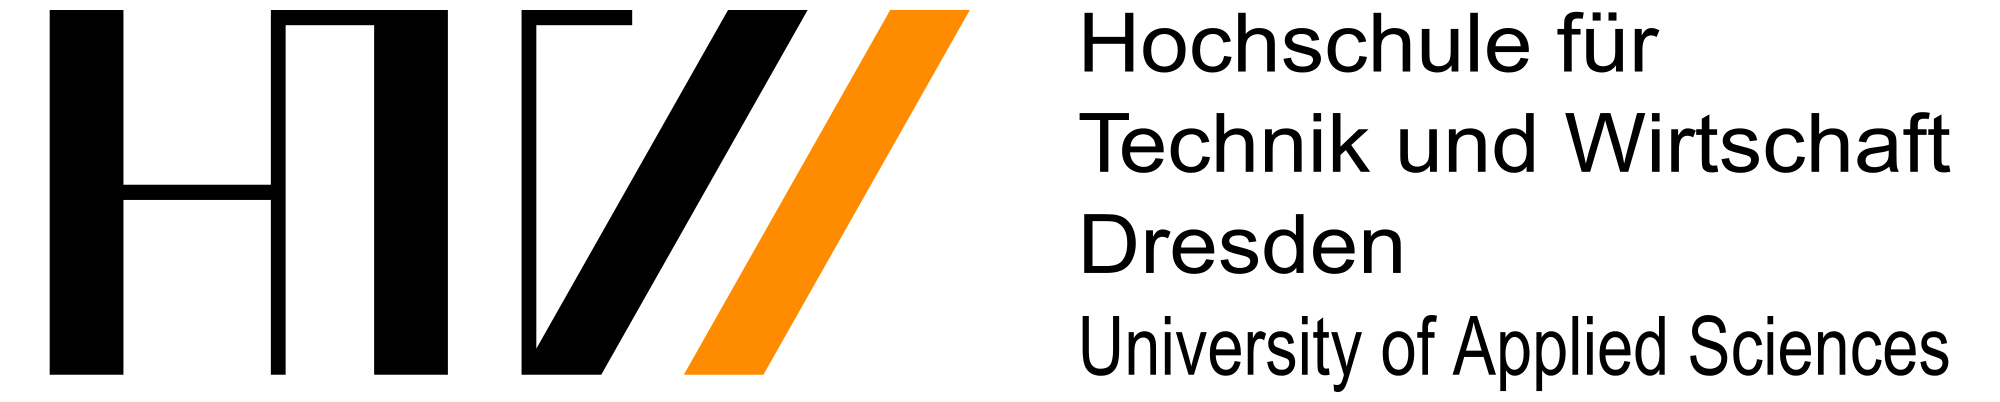
\includegraphics[width=1\textwidth]{images/HTW-Logo.png}
	\end{center}
	\Large
	\centering	
	Fakultät Informatik/Mathematik
	\mbox{}\vspace{2\baselineskip}\\
	\huge
	Diplomarbeit
	\vspace{1\baselineskip}\\
	\large
	im Studiengang Allgemeine Informatik
	\vspace{4\baselineskip}\\
	\Large
	\textbf{Thema:}\\
	\textbf{Webentwicklung mittels Kotlin am Beispiel eines RESTful-Schachservers}
	\vspace{4\baselineskip}\\
	\large
	\begin{tabular}{rl}
		Eingereicht von: & Felix Dimmel \\
		Eingreicht am: & \today \\
		Betreuer: & Prof. Dr.-Ing. Jörg Vogt \\
		2. Gutachter: & Prof. Dr.-Ing. Arnold Beck
	\end{tabular}
\end{titlepage}

%%% --- title for phd thesis --- --- --- ---
% 
% -> check your faculty documents, this is 
%    usually stipulated
